\section{Zeto}

The Zeto privacy domain consists of a collection of privacy-preserving, UTXO-based token implementations built using zero-knowledge proofs. Each Zeto token achieves a targeted subset of security properties. If the provided token implementations satisfy the security requirements for a given use case, then they can be deployed as-is. Otherwise, they can be used as templates for implementations that achieve new combinations of security goals.

This section starts by outlining the security properties targeted by Zeto tokens. We then describe how Zeto tokens achieve these properties while ensuring correctness with zero-knowledge proofs, and we illustrate how these tokens are implemented with an example.


\subsection{Preliminaries}

\subsubsection{UTXO Model}

All Zeto tokens are based on the ``unspent transaction output'' (UTXO) model~\cite{TODO}. In this model, all value is stored as records representing a certain amount of tokens that is available for a certain party to spend. We can conceptualize this as records $(\pk, v)$, where $\pk$ is the token owner's public key and $v$ is the amount of tokens they have available. A wallet will track all UTXO records corresponding to the owner's public key and enable the owner to send tokens to other users.

UTXO-based transactions are constructed functionally: each transaction has a set of input UTXOs and output UTXOs, and the sender proves ownership of the inputs by signing the transaction with their private key. The output UTXO records can be assigned to any valid public key, including that of the sender themself.

This model achieves greater scalability and throughput than tokens using an account model~\cite{TODO}, where race conditions of simultaneous transactions touching the same account must be serialized. The UTXO model avoids this problem because all unique UTXOs stay in the memory of chain nodes, and double-spending can be prevented by simply checking for uniqueness of input UTXOs within each block. However, if $(\pk, v)$ pairs are stored in plaintext on-chain, this comes at the cost of privacy, because all tokens can be linked to their owners' public keys. Additionally, the movement of tokens through transactions reveals which parties are transacting, and how much value they exchange.


\subsubsection{Zero-Knowledge Proofs}

Zero-knowledge proofs~\cite{TODO} (ZK proofs or ZKP) allow a prover to convince a verifier that a given statement is true, without the verifier learning anything except that the statement is true. For example, a prover can convince a verifier that a given transaction is valid, i.e. the sum of the input values matches the sum of the output values, without revealing any of the transaction values themselves. The prover does this by performing a computation that would be impossible (with overwhelming probability) without knowledge of all secret inputs. This type of argument is referred to as a succinct non-interactive argument of knowledge (SNARK)~\cite{TODO}. SNARKs serve as the engine underlying Zeto, enabling transaction privacy while enforcing transaction correctness in zero-knowledge. A user sending assets can generate proofs that assets are valid, and the proofs are verified on-chain by the Zeto token contract.

\paragraph{Implementation.} We implement our ZK proofs using \texttt{snarkjs}~\cite{TODO} and \texttt{circom}~\cite{TODO}. The \texttt{circom} library provides a high-level, developer-friendly syntax for specifying ZK proofs as circuits. Each proof demonstrates that a computation is performed honestly, and is represented as an arithmetic circuit over a prime-order field, with public inputs and outputs as well as private inputs. The generated proof then confirms knowledge of the secret input values such that the circuit computation is valid, without revealing any secret inputs. The \texttt{snarkjs} library provides the backend proof infrastructure that transforms a \texttt{circom} circuit and a set of inputs and outputs into a ZK proof. Several ZKP protocols to generate such proofs are available: Groth16~\cite{TODO}, PLONK~\cite{TODO}, and FFLONK~\cite{TODO}. In Zeto we use Groth16, which uses pairing-based cryptography~\cite{TODO}. This system has the smallest proof size and fastest verifier algorithm (and therefore the lowest gas costs), at the expense of slower proof generation times. Groth16 also requires a once-per-circuit trusted setup ceremony. But these backends are easily swappable, so the provided token templates can be modified to use other backends for any given use case.


\subsection{Security Goals}

% TODO: eventually add figures specifying all ZK proofs used in Zeto
% Zeto contains a *framework* for designing new privacy-preserving tokens. The pieces of Zeto ZK proofs can be combined sort of like modular blocks. Each proof contains transaction correctness validation, but can also include anonymity and any other properties that build on anonymity. I'd like to present the ZK proofs as modules somehow, with each having its own separate statement.

In this section, we describe the various security properties targeted by Zeto tokens. Each can be achieved independently, by adding a component to the ZK proof for a given token. We therefore also describe how each property is achieved within Zeto.

In addition to the below security properties, all contracts enforce transaction correctness with ZK proofs. Specifically, the proofs ensure the following.
\begin{itemize}
  \item The sum of input UTXO values is equal to the sum of the output values.
  \item All output UTXO values are positive.
  \item The sender owns private keys corresponding to public keys for all input UTXOs.
\end{itemize}

Figure~\ref{fig:zeto_proofs} contains the languages that verify each of the below security properties, as well as the language for transaction correctness.

\begin{figure*}
    \centering
    \begin{pcvstack}[boxed, center, space=2em]

      \begin{pchstack}[center, space=1em]

        \procedure{\textbf{Correctness}}{
            \\[-2ex]
            \big\{\left(\pk, (v_i, \rho_i)_{i\in [N]}, (\pk_j, v_j, \rho_j)_{j\in [M]}\right) \;\mathrm{s.t.} \\
            \t \exists\; \sk \;\mathrm{s.t.} \\
            \t \ms{PKE}.\ms{KeyGen}(\sk) = \pk \;\land \\
            \t \sum\limits_{i=1}^N v_i = \sum\limits_{j=1}^M v_j \;\land \\
            \t \forall\; j\in[M],\; v_j > 0 \big\}
        }


        \procedure{\textbf{Anonymity}}{
            \\[-2ex]
            \big\{\left(\textcolor{red}{(\ms{utxo}_i)_{i\in [N]}, (\ms{utxo}_j)_{j\in [M]}}\right) \;\mathrm{s.t.} \\
            \t \exists\; \sk \textcolor{red}{, \pk, (v_i, \rho_i)_{i\in [N]}, (\pk_j, v_j, \rho_j)_{j\in [M]}} \;\mathrm{s.t.} \\
            \t \ms{PKE}.\ms{KeyGen}(\sk) = \pk \;\land \\
            \t \sum\limits_{i=1}^N v_i = \sum\limits_{j=1}^M v_j \;\land\; \forall\; j\in[M],\; v_j > 0 \;\land \\
            \t \textcolor{red}{\forall\; i\in [N],\; \ms{utxo}_i = H(\pk, v_i, \rho_i) \;\land} \\
            \t \textcolor{red}{\forall\; j\in [M],\; \ms{utxo}_j = H(\pk_j, v_j, \rho_j)} \big\}
        }

      \end{pchstack}

      \begin{pchstack}[center, space=1em]

        \procedure{\textbf{On-chain encrypted secrets}}{
            \\[-2ex]
            \big\{\left((\ms{utxo}_i)_{i\in [N]}, (\ms{utxo}_j, \textcolor{red}{\ms{ct}_j})_{j\in [M]}\right) \;\mathrm{s.t.} \\
            \t \exists\; \sk, \pk, (v_i, \rho_i)_{i\in [N]}, (\pk_j, v_j, \rho_j)_{j\in [M]} \;\mathrm{s.t.} \\
            \t \ms{PKE}.\ms{KeyGen}(\sk) = \pk \;\land \\
            \t \sum\limits_{i=1}^N v_i = \sum\limits_{j=1}^M v_j \;\land\; \forall\; j\in[M],\; v_j > 0 \;\land \\
            \t \forall\; i\in [N],\; \ms{utxo}_i = H(\pk, v_i, \rho_i) \;\land \\
            \t \forall\; j\in [M],\; \ms{utxo}_j = H(\pk_j, v_j, \rho_j) \;\land \\
            \t \textcolor{red}{\forall\; j\in [M],\; \ms{ct}_j = \ms{PKE}.\ms{Enc}(\pk_j, (v_j, \rho_j))}\big\}
        }

        \procedure{\textbf{History masking}}{
            \\[-2ex]
            \big\{\left(\textcolor{red}{\ms{root}, (\ms{null}_i)_{i\in [N]}}, (\ms{utxo}_j)_{j\in [M]}\right), \sk \;\mathrm{s.t.} \\
            \t \exists\; \sk, \pk, (v_i, \rho_i)_{i\in [N]}, (\pk_j, v_j, \rho_j)_{j\in [M]}, \\
            \t \t \textcolor{red}{(\ms{utxo}_i)_{i\in [N]}, (\pi_i)_{i\in [N]}} \;\mathrm{s.t.} \\
            \t \ms{PKE}.\ms{KeyGen}(\sk) = \pk \;\land \\
            \t \sum\limits_{i=1}^N v_i = \sum\limits_{j=1}^M v_j \;\land\; \forall\; j\in[M],\; v_j > 0 \;\land \\
            \t \textcolor{red}{\forall\; i\in [N],\; \ms{null}_i = H(\sk, v_i, \rho_i) \;\land} \\
            \t \forall\; i\in [N],\; \ms{utxo}_i = H(\pk, v_i, \rho_i) \;\land \\
            \t \textcolor{red}{\forall\; i\in [N], \ms{SMT}.\ms{Verify}(\ms{root}, (\ms{utxo}_i, \ms{utxo}_i), \pi_i) = 1 \;\land} \\
            \t \forall\; j\in [M],\; \ms{utxo}_j = H(\pk_j, v_j, \rho_j) \big\}
        }

      \end{pchstack}

      \begin{pchstack}[center, space=1em]

        \procedure{\textbf{Know Your Customer}}{
            \\[-2ex]
            \big\{\left((\ms{utxo}_i)_{i\in [N]}, (\ms{utxo}_j)_{j\in [M]}\right) \;\mathrm{s.t.} \\
            \t \exists\; \sk, \pk, (v_i, \rho_i)_{i\in [N]}, (\pk_j, v_j, \rho_j)_{j\in [M]} \textcolor{red}{, \ms{root}, \pi} \;\mathrm{s.t.} \\
            \t \ms{PKE}.\ms{KeyGen}(\sk) = \pk \;\land \\
            \t \textcolor{red}{\ms{SMT}.\ms{Verify}(\ms{root}, (\pk, \pk), \pi) = 1 \;\land} \\
            \t \sum\limits_{i=1}^N v_i = \sum\limits_{j=1}^M v_j \;\land\; \forall\; j\in[M],\; v_j > 0 \;\land \\
            \t \forall\; i\in [N],\; \ms{utxo}_i = H(\pk, v_i, \rho_i) \;\land \\
            \t \forall\; j\in [M],\; \ms{utxo}_j = H(\pk_j, v_j, \rho_j)\big\}
        }

        \procedure{\textbf{Non-repudiation}}{
            \\[-2ex]
            \big\{\left((\ms{utxo}_i)_{i\in [N]}, (\ms{utxo}_j)_{j\in [M]} \textcolor{red}{, \ms{ct}} \right) \;\mathrm{s.t.} \\
            \t \exists\; \sk, \pk, (v_i, \rho_i)_{i\in [N]}, (\pk_j, v_j, \rho_j)_{j\in [M]} \;\mathrm{s.t.} \\
            \t \ms{PKE}.\ms{KeyGen}(\sk) = \pk \;\land \\
            \t \textcolor{red}{\ms{ct} = \ms{PKE}.\ms{Enc}(\pk_\ms{audit}, (\pk, (v_i, \rho_i)_{i\in [N]}, (\pk_j, v_j, \rho_j)_{j\in [M]})) \;\land} \\
            \t \sum\limits_{i=1}^N v_i = \sum\limits_{j=1}^M v_j \;\land\; \forall\; j\in[M],\; v_j > 0 \;\land \\
            \t \forall\; i\in [N],\; \ms{utxo}_i = H(\pk, v_i, \rho_i) \;\land \\
            \t \forall\; j\in [M],\; \ms{utxo}_j = H(\pk_j, v_j, \rho_j)\big\}
        }

      \end{pchstack}
    \end{pcvstack} % TODO: this figure is a bit too wide because of the non-repudiation language. Maybe this is fixable later.
    \caption{Collection of languages verified by zero-knowledge proofs to achieve Zeto privacy goals. In this notation, public inputs (the statement) are on the first line, and secret inputs (the witness) are on the second line. Additional components and modifications over standard anonymity are shown in \textcolor{red}{red}. For the anonymity language, red components are additional to standard correctness.}
    \label{fig:zeto_proofs}
\end{figure*}


\paragraph{Anonymity.} This property ensures that no transaction reveals which user maintains ownership of a particular UTXO. All other security goals for Zeto tokens assume anonymity. For example, masking transaction history does not make sense unless the contents of each transaction are also masked.

To achieve this property, ownership of a particular UTXO is tied not to the \texttt{msg.sender} of a transaction, but to a private key stored off-chain. In this way, users can generate fresh signing keys for each EVM transaction without ever revealing the public key tied to a UTXO. We also only store \textit{commitments} to Zeto UTXOs on-chain, rather than the contents of the UTXO themselves. Each commitment is instantiated as a salted hash of a pair $(\pk, v)$, with salt $\rho$. In each token transfer, senders provide commitments to input and output UTXOs, and generate a SNARK to prove knowledge of the following values:
\begin{itemize}
  \item $(\pk, v_i)$ and salt values $\rho_i$ that constitute valid pre-images of each input commitment $i$.
  \item $(\pk_j, v_j)$ and salt values $\rho_j$ that constitute valid pre-images of each output commitment $j$.
\end{itemize}

The contract maintains a list of all valid UTXO commitments, and marks them as spent as they are consumed to prevent double-spending. When the Zeto contract verifies this proof, it is convinced that the input and output commitments that it sees commit to a set of UTXOs that form a valid transaction. The sender can then reveal output UTXO information to the receivers out-of-band so they can use the committed-to UTXOs in future transactions. Note that anonymity (as described here) \textit{does not} hide relationships between input and output UTXOs. All UTXOs have a fixed salt and a fixed commitment stored on-chain. Unlinkability between any UTXOs in a given transaction is achieved by using nullifiers, as described below under \textit{history masking}.

\paragraph{On-chain encrypted secrets.} In isolation, satisfying anonymity (as described above) requires senders to reveal the output UTXOs to their respective receivers out-of-band. If a Zeto token only implements anonymity, a malicious sender could generate a valid transaction (consuming UTXOs that they own) but simply not reveal the output UTXOs to the intended recipients. Zeto provides ZK proofs and contracts that not only enforce honesty in the anonymous setting, but also require that the sender encrypts output UTXOs for the intended recipients so that these ciphertexts can be stored on-chain. Therefore sender honesty is enforced by auditability of the underlying blockchain and soundness of the ZKP scheme.

% uses poseidon encryption
% encrypts the output UTXO information: the tx value and salt for the UTXO
% No additional privacy over "anonymity". the difference is that here we store encryptions of the output UTXO values and salts on the base chain.
% don't rely on off-chain channels for receivers to get necessary secrets
% malicious sender can't hide the sent tokens from the receiver

\paragraph{History masking.} This property further guarantees that no party can identify which UTXOs are input to any transaction. In effect, this hides the history of a particular quantity of tokens, as the inputs and outputs of a transfer are unlinkable and their connection is not revealed on-chain.

History masking is implemented using nullifiers~\cite{TODO}. For a UTXO computed as $H(\pk, v, \rho)$, its nullifier is the quantity $H(\sk, v, \rho)$, where $(\sk, \pk)$ is a valid key pair. The nullifier is a quantity that only the token owner can compute, but by the hiding of this commitment scheme, does not reveal either $\sk$ or $v$. At transfer time, the sender provides nullifiers corresponding to each input UTXO, and proves knowledge of corresponding UTXOs and their commitments. Then to prove that these UTXOs are valid, the sender also proves knowledge of merkle proofs that each of these UTXOs are in a merkle tree with a root maintained by the token contract. The contract then checks whether the provided root is one of the historical ones it's maintained, and if so it verifies and accepts the proof.

Note that in order to use nullifiers, the client must maintain state representing the merkle tree of UTXO commitments so that it can generate merkle proofs. To prevent race conditions and improve transaction throughput, we allow the provided merkle root to be historical, as long as it was valid at some point. This storage can also be optimized significantly: because clients only use portions of the merkle tree surrounding their own transactions, they can ignore all other portions and still generate valid proofs. This means clients only need to store data of size linear in the number of UTXOs they own and logarithmic in the size of the tree.

\paragraph{Know Your Customer (KYC).} Financial institutions often have policy or legal requirements that enforce verification of customers' identities. In this setting, we define KYC as the property that clients are able to prove membership to a list of vetted clients, without revealing their identity. For example, the platform maintaining a KYC Zeto contract could verify the ID of a user, and then add their client's public key to a merkle tree containing vetted clients. Our KYC contracts do just this. Clients prove (in zero-knowledge) ownership of a secret key corresponding to a public key with a valid merkle proof, relative to the merkle tree of client identities.

\paragraph{Non-repudiation.} For regulatory or policy reasons, a token may also need to be auditable to an auditing authority. Non-repudiation requires that all transactions are auditable, i.e. users can't deny to the auditor that a particular transaction took place. To achieve non-repudiation while maintaining anonymity, we require users to encrypt a record of each transaction to the auditor, which is stored on-chain. This record includes owner identities, transaction values, and salts for each input and output UTXO commitment. We use the Poseidon encryption system, and augment our ZK proof to verify that the ciphertext encrypts the correct plaintext. Therefore non-repudiation is guaranteed by the soundness of the ZKP scheme.

\paragraph{Post-quantum security.} Large-scale quantum computers have the potential to compromise a large number of cryptographic primitives. As described above, Poseidon encryption for non-repudiation uses the Diffie-Hellman key exchange~\cite{TODO} to arrive at a shared secret key. While this is highly efficient, it relies on the hardness of the discrete logarithm problem~\cite{TODO}, for which known quantum attacks exist. While cryptographically relevant quantum computers are likely decades away, progress in the field can enable ``harvest now, decrypt later'' attacks~\cite{TODO}. Any ciphertexts sent today with quantum-insecure encryption may be stored until a quantum computer is powerful enough to decrypt them. This is why highly sensitive applications are beginning to transition to post-quantum encryption, and why NIST is deprecating some lower-security versions of Diffie-Hellman as early as 2030~\cite{TODO}.

To address this, Zeto includes tokens that achieve the same properties as non-repudiation tokens, but establish a shared secret using the NIST-standardized ML-KEM key establishment scheme~\cite{TODO}.

% encrypts tx info (input and output owner, input and output values and salts) to be decrypted by an authority
% identical to qurrency but not post-quantum secure < ** maybe note qurrency here **

% \begin{figure*}
%     \centering
%     \begin{pchstack}[boxed, center, space=1em]

%         \procedure{$\ms{CORRECT}[\calA, \calT, U, N, M, \lambda]$}{
%             \\[-2ex]
%             \ms{ks} \gets \calA \\
%             \pcassert \ms{len}(\ms{ks}) = U \\
%             \pcfor i \in [U]: \\
%             \t \sk_i, \pk_i \gets \ms{ks}[i] \\
%             \t \pcassert \pk_i = \ms{PKE}.\ms{KeyGen}(\sk_i) \\
%             b' \gets \calA^{\calO_{\ms{SendTx}}}(1^\lambda) \\
%             \ms{output}\; b'
%         }

%         \procedure{$\calO_\ms{SendTx}(\ms{sender}, \ms{tx})$}{
%             \\[-2ex]
%             (\ms{utxo}_i)_{i\in [N]}, (\ms{utxo}_j)_{j\in [M]}, \pi \gets \ms{tx} \\
%             \pcassert \ms{ZK}.\ms{Verify}\left(\pi, (\ms{utxo}_i)_{i\in [N]}, (\ms{utxo}_j)_{j\in [M]}\right) = 1 \\
%             \sk, \pk, (v_i, \rho_i)_{i\in [N]}, (\pk_j, v_j, \rho_j)_{j\in [M]} \gets \ms{witness}_\ms{tx} \\
%             \pcfor i \in [N]: \\
%             \t \pcassert \ms{utxo}_i = 
%         }

%     \end{pchstack}
%     \caption{}
%     \label{}
% \end{figure*}

\subsection{Security definitions and arguments}

\paragraph{Transaction Correctness.} This property ensures that each transaction is well-formed. Specifically, we require the following.
\begin{itemize}
  \item The sum of the input UTXO values is equal to the sum of the output UTXO values.
  \item All output values are positive.
  \item The transaction sender has knowledge of a $\sk$ such that all input UTXOs belong to the corresponding $\pk$.
  \item All input UTXOs exist and are unspent.
  \item All output UTXOs do not yet exist.
\end{itemize}

For all Zeto tokens, the first three requirements follow directly from soundness of the ZKP scheme, and from the inclusion of correctness clauses in each token's ZKP language. If a given transaction verifies, the contract is convinced (with high probability) that the transaction is valid.

How the smart contract enforces the fourth requirement varies by token. For Zeto tokens without history masking, this are enforced by the contract itself. In this setting, since all input and output UTXO commitments are revealed publicly, the contract maintains a list of all UTXOs for the given token ecosystem. If the proof for a transaction is accepted, the contract can lookup all input UTXO commitments to ensure that they exist and are unspent, and it can lookup all output UTXO commitments to ensure that they do not yet exist. It can then update the spent status of each UTXO touched in the transfer. Therefore in this case, the final two transaction correctness requirements follow from correctness of the smart contract logic.

For Zeto tokens with history masking, the contract is unable to perform these checks on input UTXO commitments, because the commitments are not revealed publicly. (It can, however, verify that the revealed output UTXOs do not yet exist.) Therefore input UTXOs are validated within the ZK proof. The sender proves knowledge of UTXO commitments corresponding to each publicly revealed nullifier, and also proves knowledge of merkle proofs that confirm each UTXO commitment's membership within a sparse merkle tree which has the revealed \ms{root}. Furthermore, since each nullifier is a deterministic function of a UTXO's $(\sk, v, \rho)$, each UTXO can only be nullified once. In order to be convinced that each input UTXO exists and is unspent, the contract only needs to verify the proof, and mark all input nullifiers as consumed. Therefore the final two transaction correctness requirements follow from soundness of the ZKP scheme and correctness of the smart contract logic.

\paragraph{Privacy Goals.} % follows directly from zero-knowledge
Each language shown in Figure~\ref{fig:zeto_proofs} enforces a specific security or privacy goal. Privacy goals ensure that some subset of the transaction information (shown as public signals in the ``Correctness'' language in Figure~\ref{fig:zeto_proofs}) are hidden on-chain. For example, anonymity ensures that all public keys, values, and salts are not revealed on-chain, and instead only commitments to these values are revealed. History masking goes further, and ensures that not even commitments to the input values are revealed on-chain. These privacy goals all follow directly from the zero-knowledge property of the underlying ZKP scheme.

\subsection{Example Token: \texttt{anon\_nullifier\_kyc}}

A block diagram representing the zero-knowledge proof circuit for the \texttt{anon\_nullifier\_kyc} token is shown in Figure~\ref{fig:zeto_circuit}. In this section, we further highlight how information is processed in this circuit, and how different components of the circuit enforce our desired privacy and security properties. Throughout the section, we will refer to subroutines of the circuit in Figure~\ref{fig:zeto_circuit} as the first, second, etc. blocks. This ordering is defined top to bottom, left to right.

All inputs that the prover needs are shown on the left. Private inputs (those that are hidden from the perspective of the verifier) are shown in orange, and publicly revealed inputs are shown in teal. Output bits are on blue wires. These are the results of assertions: if all output bits are 1, then the circuit has confirmed that the supplied inputs form a valid transaction.

The first three blocks of the diagram ensure \textit{transaction correctness}. The first asserts that all output UTXO values are positive, and the second asserts that the sum of the input values equals the sum of the output values. The third computes an internal signal containing the public key corresponding to the provided secret key. These components are common to all Zeto tokens.

The fourth and fifth blocks enforce the \textit{anonymity} requirements of the ZK proof, and correspond to the red components of the anonymity language in Figure~\ref{fig:zeto_proofs}. They assert that the commitments to input and output UTXO data is well-formed. Note that, because this circuit provides history masking, only the output UTXO commitments are revealed. The input UTXO commitments are a private input to the circuit, not seen by the verifier.

The sixth and seventh blocks enforce \textit{history masking}. The sixth ensures that the publicly revealed nullifiers are well-formed. We require not only that each nullifier is computed as $H(\sk, v_i, \rho_i)$, but crucially, these should be the same $(v_i, \rho_i)$ pairs corresponding to the hidden input commitments, and $\sk$ is the secret key corresponding to the public key $\pk$ contained in the input commitments. This links each nullifier to a corresponding UTXO commitment. Then the seventh block verifies that those hidden input commitments are in fact valid members of a sparse merkle tree. It does this without revealing the input commitments, nor the proofs themselves. Only the merkle root is revealed. If these assertions pass, without learning anything else, the verifier can be convinced that the prover knows a set of input UTXOs such that (a) the prover knows the secret key for these UTXOs, and (b) the prover knows a valid proof that commitments to these UTXOs are stored in the merkle tree with the provided root.

Finally, the last three blocks enforce \textit{KYC}. The mechanism here is very similar to that used in the history masking components. But here, the elements of the merkle tree are commitments to user identities. In practice, the Zeto maintainer would apply out-of-band customer vetting before adding any customer to the identity merkle tree. Therefore, if the transaction sender can prove knowledge of a valid merkle proof that the sender and all receivers have identities that are members of this SMT, the verifier is convinced that all customers have been vetted, without learning any information except the revealed merkle root.

\begin{figure*}
\centering
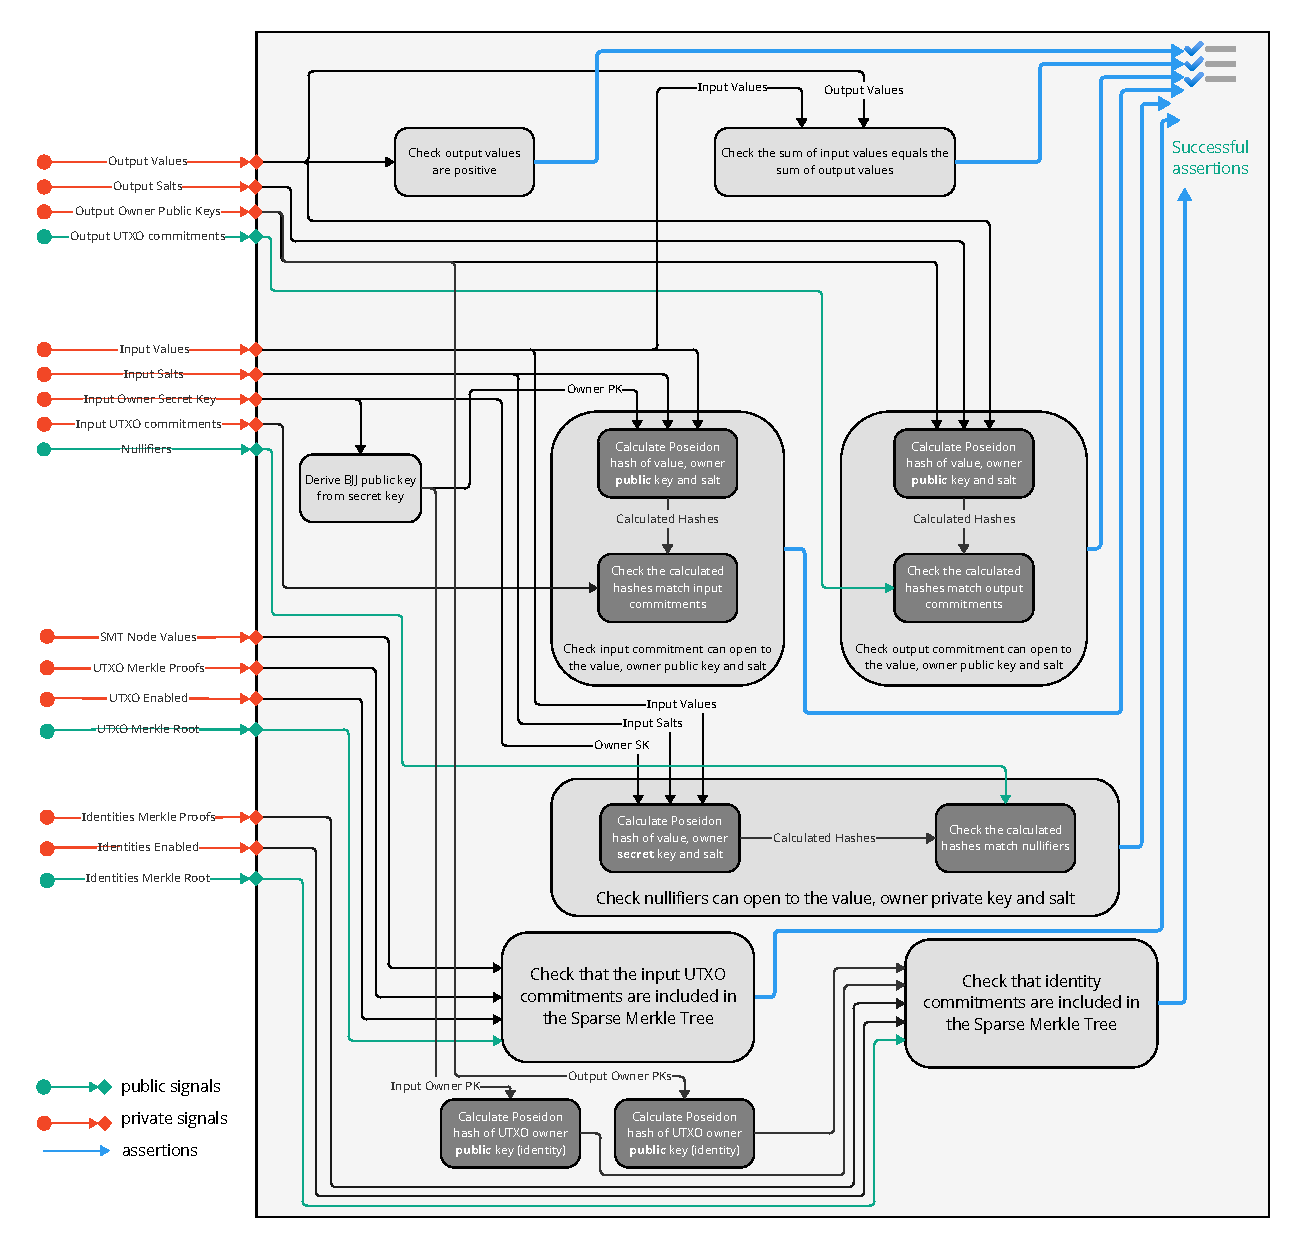
\includegraphics[width=\linewidth]{anon_nullifier_kyc.pdf}
\caption{Block diagram of the circuit verified by the zero-knowledge proof for the \texttt{anon\_nullifier\_kyc} Zeto token.}\label{fig:zeto_circuit}
\end{figure*}

% reiterate points from "preliminaries": ZK proof ensures honest transaction generation, but only a subset of the values are revealed publicly